\documentclass[10pt]{beamer}
\usetheme{jambro}

\title[]{Pensamento Econômico Contemporâneo - A escola monetarista ortodoxa}
\author[]{Paulo Victor da Fonseca}
\date{}

\hypersetup{
    colorlinks = true,
    urlcolor = teal,
    linkcolor = teal    
}
\usepackage[portuguese]{babel}
\usepackage{subfig}
\usepackage{emoji}

\begin{document}

\begin{frame}[plain]
    \titlepage{
        \begin{center}
            \begin{minipage}{0.8\textwidth}
                \centering
            \end{minipage}
        \end{center}}
\end{frame}

\begin{frame}{Sumário}
    \tableofcontents
\end{frame}

\section{Proposições centrais (Keynesiana)}
\begin{frame}{Proposições centrais da economia Keynesiana}
    \begin{enumerate}
        \item[P1.] Economias sujeitas a falha endêmica, dado que são propensas a custosas recessões que são, primariamente, causadas por deficiência de demanda (efetiva) agregada
        \bigskip
        \begin{itemize}
            \item Recessões vistas como desvios indesejados do equilíbrio de pleno emprego, geralmente causados por choques de demanda (fatores diversos reais e monetários)
            \medskip
            \item Contraste com \textcolor{purple}{teoria dos ciclos reais de negócios}: choques de oferta como causas principais de instabilidade agregada
        \end{itemize}
    \end{enumerate}
\end{frame}

\begin{frame}{Proposições centrais da economia Keynesiana}
    \begin{enumerate}
        \item[P2.] Keynesianos ortodoxos: dois possíveis regimes na economia. \textcolor{blue}{Regime Keynesiano} - atividade econômica agregada restringida pela demanda. \textcolor{blue}{Regime clássico} - produto restringido pela oferta e lei de Say é válida
        \bigskip
        \begin{itemize}
            \item Visão Keynesiana `antiga': economia pode estar em qualquer um destes regimes em pontos distintos do tempo
            \medskip
            \item \textcolor{purple}{Economia novo-clássica}: sistema econômico modelado como se estivesse sempre em regime restrito pela oferta
            \medskip
            \item No regime Keynesiano, \textcolor{blue}{emprego e produto respondem positivamente a demandas reais adicionais, independente de qual seja a origem}
        \end{itemize}
    \end{enumerate}
\end{frame}

\begin{frame}{Proposições centrais da economia Keynesiana}
    \begin{enumerate}
        \item[P3.] Desemprego é uma característica central ao regime Keynesiano, e a maior parte deste desemprego é involuntário.
        \bigskip        
    \end{enumerate}
    \begin{itemize}
        \item Esta visão contrasta com grande parte da escola \textcolor{purple}{monetarista, novo-clássica e teoria dos ciclos reais de negócios} - desemprego é um fenômeno voluntário.
    \end{itemize}
\end{frame}

\begin{frame}{Proposições centrais da economia Keynesiana}
    \begin{enumerate}
        \item[P4.] \NB{Uma economia de mercado \'{e} sujeita a flutua\c{c}\~{o}es no produto agregado, desemprego e pre\c{c}os, que precisam ser corrigidos, podem ser corrigidos e, portanto, deveriam ser corrigidos (Modigliani, 1977, 1986)}
        \bigskip
        \begin{itemize}
            \item O uso discricionário e coordenado de políticas fiscal e monetária tem papel importante na estabilização da economia
            \bigskip
            \item Estes instrumentos macroeconômicos devem ser orientados a objetivos econômicos reais - produto real e emprego
            \bigskip
            \item Keynesianos `fiscalistas' (termo não muito apropriado) para distinguir dos monetaristas
        \end{itemize}
    \end{enumerate}
\end{frame}

\begin{frame}{Proposições centrais da economia Keynesiana}
    \begin{enumerate}
        \item[P5.] Preços e salários não são perfeitamente flexíveis. Portanto, mudanças de DA - antecipadas ou não - vão ter um impacto direto maior no curto prazo sobre o produto real e emprego do que sobre variáveis nominais
        \medskip
        \begin{itemize}
            \item Dadas as rigidezes nominais de preço, a curva de oferta agregada de curto prazo é positivamente inclinada, pelo menos até a economia atingir o equilíbrio de pleno emprego restrito pela oferta
        \end{itemize}
        \bigskip
        \item[P6.] Ciclos de negócios representam flutuações no produto que são desvios indesejáveis abaixo do de trajetória de tendência de equilíbrio de pleno emprego do produto. Ciclos de negócios não são flutuações simétricas ao redor da tendência
    \end{enumerate}
\end{frame}

\begin{frame}{Proposições centrais da economia Keynesiana}
    \begin{enumerate}
        \item[P7.] Formuladores de política econômica que controlam as políticas fiscal e monetária se deparam com um trade-off não linear entre inflação e desemprego no curto prazo
        \bigskip
        \begin{itemize}
            \item Década de 1960: crença em um trade-off relativamente estável
            \medskip
            \item Solow e Tobin (1988) admitiram que no início dos anos 60 eles podem ter `apostado' demais na estabilidade da curva de Phillips indicada pelos dados do pós-guerra até 1961'
        \end{itemize}
    \end{enumerate}
\end{frame}

\begin{frame}{Proposições centrais da economia Keynesiana}
    \begin{enumerate}
        \item[P8.] Macro Keynesiana: problemas de instabilidade de curto prazo, sem pretensões de ser aplicável às questões de crescimento e desenvolvimento de longo prazo
        \bigskip
        \begin{itemize}
            \item Separação de flutuações de curto prazo de demanda das tendências de longo prazo caracterizadas pela oferta é uma das principais características da síntese neoclássica
            \medskip
            \item No entanto, políticas de estabilização que combinam uma política fiscal rígida com uma política monetária flexível levarão a ``um mix de produto com peso maior sobre o investimento e formação de capital, e menor sobre o consumo''
            \medskip
            \item Esse mix, portanto, será mais propício para elevações do crescimento do PIB potencial de longo prazo de uma economia
            \medskip
            \item \NB{Controlar o ciclo de neg\'{o}cios e manter o pleno emprego s\~{a}o as principais prioridades das pol\'{i}ticas macroecon\^{o}micas. Mas isso deve ser feito de forma a promover um crescimento mais r\'{a}pido na capacidade produtiva da economia (Tobin, 1996)}
        \end{itemize}
    \end{enumerate}
\end{frame}

\section{Monetarismo}
\subsection{Introdução}
\begin{frame}{Introdução}
    \begin{itemize}
        \item Dominância teórica e de prescrição de política da macro Keynesiana - com modelo IS/LM - durante 1950s e 1960s
        \bigskip
        \item Teoria Geral: economias capitalistas de mercado são inerentemente instáveis e podem convergir para um equilíbrio estável abaixo do pleno emprego por um longo período de tempo
        \bigskip
        \item Instabilidade predominantemente resultado de flutuações de DA
        \bigskip
        \item Anos 40 e 50: Keynesianos dão ênfase a distúrbios reais (flutuações no investimento e consumo autônomo) como principais causas para flutuações na moeda e renda nominal, predominantemente sob a forma de variações na renda real
    \end{itemize}
\end{frame}

\begin{frame}{Introdução}
    \begin{itemize}
        \item Para Keynesianos, a Grande Depressão foi resultado de um declínio acentuado do nível de investimento com o desemprego severo associado refletindo um estado de deficiência de DA
        \bigskip
        \item Contraste com TQM: $\Delta$ estoque de moeda fator predominante, apesar de não único, na explicação de $\Delta$ renda nominal
        \bigskip
        \item Durante as décadas de 1950s e 1960s, Milton Friedman foi o responsável por `reviver' a TQM - a plataforma central do \textcolor{purple}{monetarismo}
    \end{itemize}
\end{frame}

\begin{frame}{Introdução}
    \begin{itemize}
        \item Nosso objetivo é traçar o desenvolvimento histórico do \textcolor{purple}{monetarismo ortodoxo} - Figura \ref{fig1}:
        \bigskip
        \begin{enumerate}
            \item A abordagem da \hlight{Teoria Quantitativa da Moeda} e sua evolução nos anos 50s e 60s
            \medskip
            \item Análise da \hlight{curva de Phillips aumentada por expectativas} que foi incorporada à escola monetarista no final dos anos 60s
            \medskip
            \item A abordagem monetarista da teoria de balanço de pagamentos e determinação da taxa de câmbio
        \end{enumerate}
        \bigskip
        \item Além disso, resumir as principais características que distinguem a escola monetarista ortodoxa
        \bigskip
        \item Especialmente papel e condução de políticas de estabilização e avaliar o que ainda permanece no pensamento macro atual da contra-revolução monetarista
    \end{itemize}
\end{frame}

\begin{frame}{Introdução}
    \begin{figure}
        \centering
        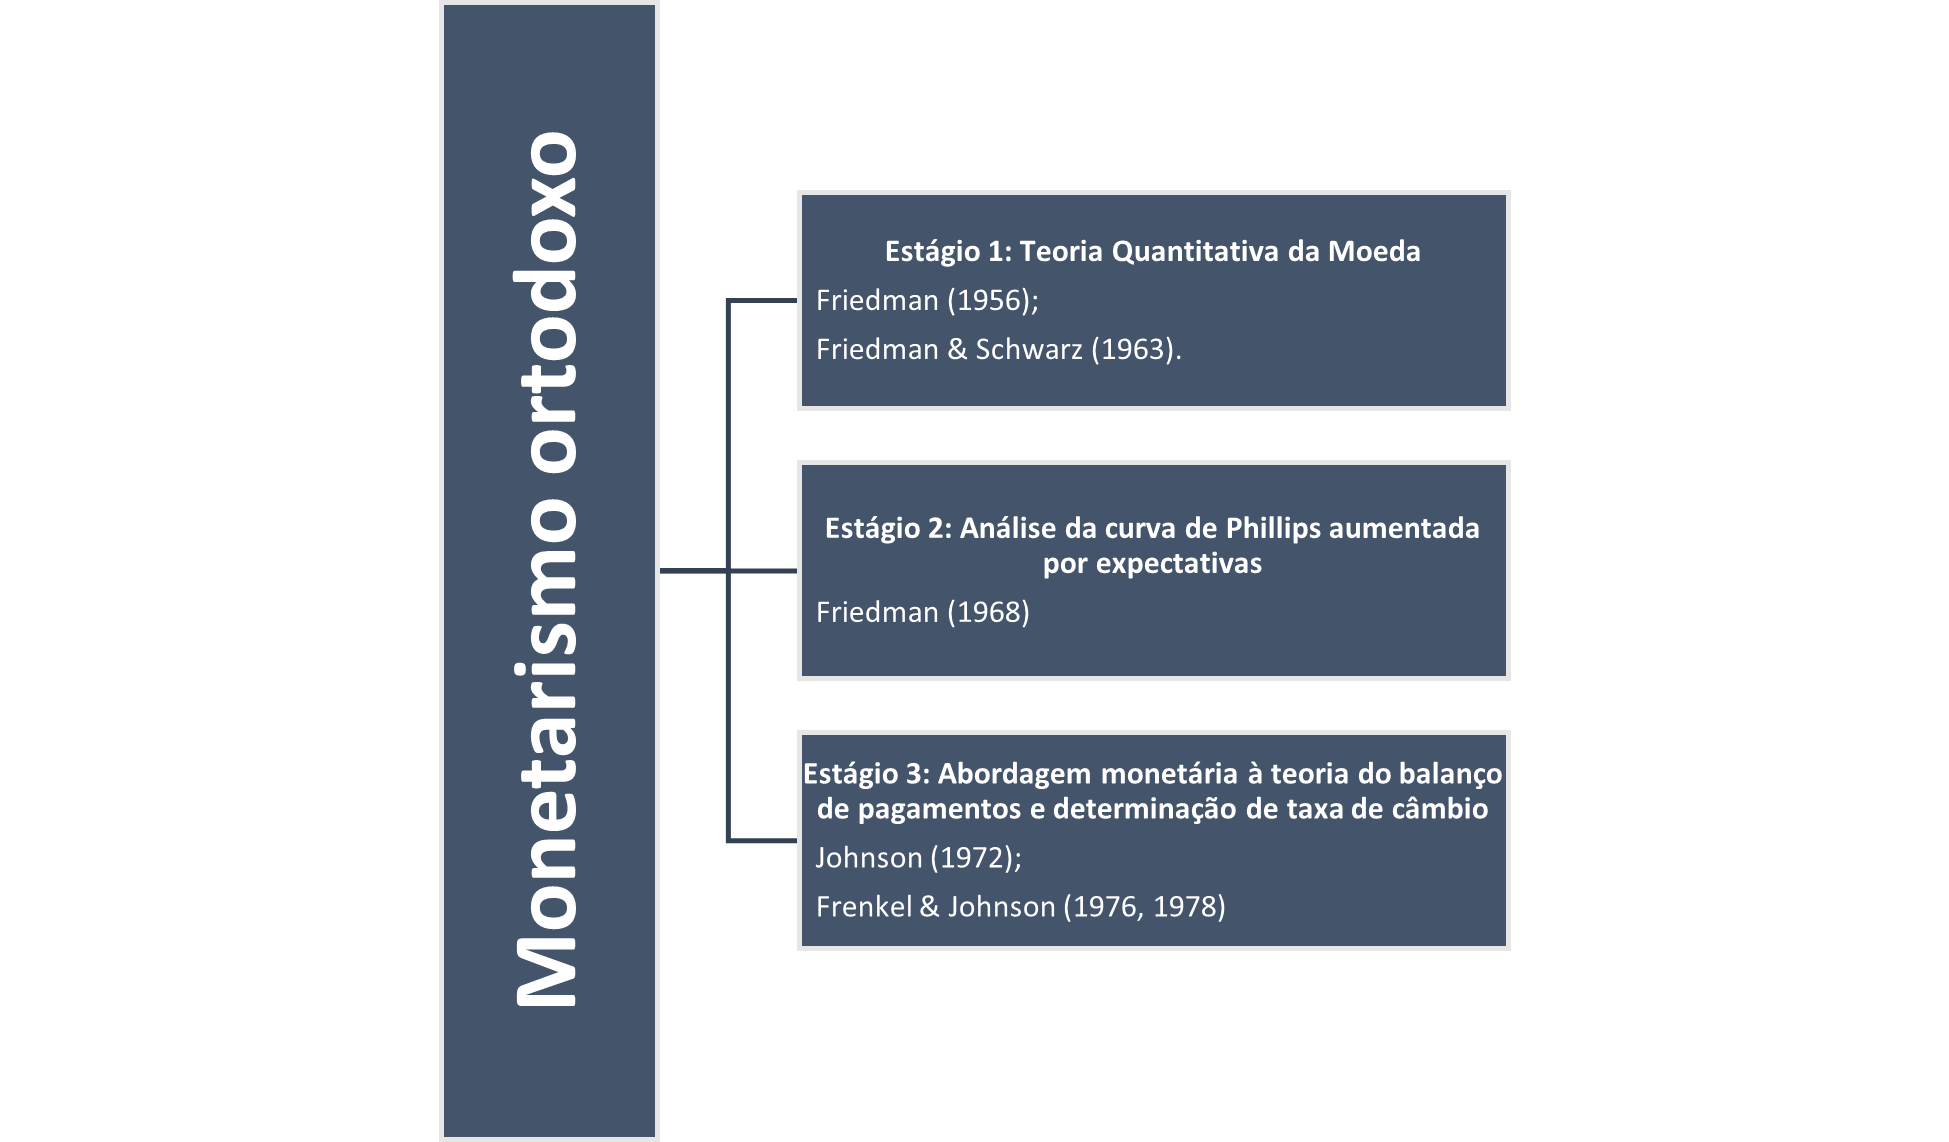
\includegraphics[width=0.75\textwidth]{./figures/aula9_fig1.png}
        \caption{Evolução do monetarismo ortodoxo. Fonte: Snowdon e Vane (2005).}
        \label{fig1}
    \end{figure}
\end{frame}

\section{Teoria Quantitativa da Moeda}
\subsection{Introdução}
\begin{frame}{Introdução}
    \begin{itemize}
        \item Primeiro estágio (1950s e 1960s): tentativa de reestabelecer a TQM na análise macro
        \bigskip
        \item Em termos da TQM estilizada que estudamos no modelo clássico, a Teoria Geral de Keynes foi interpretada como implicando que em condições de subemprego, a velocidade-renda da moeda ($V$) seria altamente instável e se ajustaria de maneira passiva a qualquer variação que viesse a ocorrer de maneira independente na oferta de moeda ($M$) ou na renda nominal ($PY$)
        \bigskip
        \item Neste contexto, a moeda é relativamente sem importância \bigskip
        \item E.g.: sob armadilha de liquidez ou investimento inelástico, a moeda não importa tanto, já que a política monetária seria completamente ineficaz em influenciar o nível de atividade econômica
    \end{itemize}
\end{frame}

\begin{frame}{Introdução}
    \begin{itemize}
        \item Armadilha da liquidez: aumento na oferta de moeda seria completamente compensado por uma variação na direção oposta da velocidade da moeda
        \bigskip
        \item O aumento na oferta de moeda seria inteiramente absorvido sob a forma de encaixes especulativos/ociosos com uma taxa de juros e nível de renda constantes
        \bigskip
        \item Armadilha do investimento (investimento completamente inelástico): aumento na oferta de moeda também não teria efeito algum sobre o nível de renda real
        \bigskip
        \item A velocidade reduziria à medida que a demanda por moeda aumenta relativamente a um nível de renda inalterado \bigskip
        \item Nessas condições, TQM permanece válida mas Keynesianos argumentam que seria inútil prescrições de política econômica em termos de política monetária
    \end{itemize}
\end{frame}

\subsection{A teoria quantitativa como uma teoria de demanda por moeda}
\begin{frame}{TQM como uma teoria de demanda por moeda}
    \begin{itemize}
        \item Friedman: reabilitação da TQM $\times$ ortodoxia Keynesiana
        \bigskip
        \item Transformar a equação tautológica de quantidade de moeda da TQM clássica em uma equação de demanda por moeda
        \bigskip
        \item Lembrando da TQM Fisheriana de equação de trocas expressa em termos de renda, temos:
        \[
        M^sV = PY,
        \]
        onde $M^s$ é a oferta de moeda (igual ao estoque), $V$ a velocidade-renda, $P$ o nível de preços e $Y$ o produto agregado real
    \end{itemize}
\end{frame}

\begin{frame}{TQM como uma teoria de demanda por moeda}
    \begin{itemize}
        \item $PY$ pode ser interpretado, portanto, como renda ou PIB nominal
        \bigskip
        \item A velocidade-renda da moeda ($V \equiv PY/M$) é, então, a fração de renda nominal adquirida por cada unidade monetária ao longo de um intervalo temporal
        \bigskip
        \item Como vimos, a hipótese de Fisher era de que velocidade e produto são constantes no curto prazo - variações na quantidade de moeda resulta em variações proporcionais no nível de preços:
        \[
        M\bar{V} = P\bar{Y}
        \]
        \bigskip
        \item A mesma relação pode ser obtida com a equação de encaixes monetários de Cambridge (que possui um fundamento comportamental mais sólido):
        \[
        M^d = kPY,
        \]
        onde $k$ é um fator de proporcionalidade entre a demanda por moeda e a renda nominal
    \end{itemize}
\end{frame}

\begin{frame}{TQM como uma teoria de demanda por moeda}
    \begin{itemize}
        \item Para que a noção de equilíbrio no mercado monetário faça sentido, as funções de oferta de moeda e demanda por moeda devem ser independentes
        \bigskip
        \item De acordo com Friedman, a oferta monetária refere-se ao estoque \textcolor{blue}{nominal} de moeda
        \bigskip
        \item Friedman e Schwartz identificaram três determinantes para este estoque:
        \bigskip
        \begin{enumerate}
            \item Base monetária restrita
            \bigskip
            \item A razão de reservas dos bancos comerciais
            \bigskip
            \item A razão depósitos/moeda em poder do público
        \end{enumerate}
        \bigskip
        \item Friedman e Schwartz adotam a premissa tradicional de que a oferta de moeda é exógena
    \end{itemize}
\end{frame}

\begin{frame}{TQM como uma teoria de demanda por moeda}
    \begin{itemize}
        \item Objetivo: fundamentar uma teoria de demanda por moeda, referindo-se à quantidade \textcolor{blue}{real} de moeda (ou `encaixes reais') que agentes econômicos otimizadores desejam reter
        \bigskip
        \item Friedman postulou que a demanda por moeda (como a demanda por qualquer ativo) fornece um fluxo de serviços ao seu detentor e depende, essencialmente, de três fatores principais:
        \bigskip
        \begin{enumerate}
            \item A restrição de riqueza, que determina a quantidade máxima de moeda que pode ser retida por um agente
            \medskip
            \item O retorno da moeda em relação ao retorno de outros ativos financeiros e reais sob os quais a riqueza pode ser alocada
            \bigskip
            \item As preferências e gostos do detentor de ativos
        \end{enumerate}
    \end{itemize}
\end{frame}

\begin{frame}{TQM como uma teoria de demanda por moeda}
    \begin{itemize}
        \item A forma com que a riqueza total é alocada entre as várias formas de ativos depende das taxas de retorno relativas entre estes ativos
        \bigskip
        \item Estes ativos incluem não só a moeda e os títulos mas, também, ações e bens físicos
        \bigskip
        \item No equilíbrio, a riqueza será alocada entre ativos de forma que as taxas marginais de retorno sejam equalizadas
        \bigskip
        \item Apesar de Patinkin (1969) argumentar que a reinterpretação de Friedman possa ser considerada uma extensão da análise de demanda por moeda de Keynes, três distinções importantes merecem ser mencionadas:
        \bigskip
        \begin{enumerate}
            \item A teoria de demanda por moeda de Friedman pode ser considerada uma aplicação de sua teoria de consumo e a \textcolor{blue}{hipótese da renda permanente} para um ativo particular
            \medskip
            \item Friedman introduz a expectativa de taxa de inflação como uma variável potencialmente importante
            \medskip
            \item A demanda por moeda é uma função estável de um número limitado de variáveis
        \end{enumerate}
    \end{itemize}
\end{frame}

\begin{frame}{TQM como uma teoria de demanda por moeda}
    \begin{itemize}
        \item Uma versão simplificada da função de demanda por encaixes reais pode ser escrita da seguinte forma:
        \begin{equation}
            \frac{M^d}{P} = \Phi\left(Y^p, k(R_B - R_M, R_E-R_M, \pi^e-R_M); u\right),
            \label{eq1}
        \end{equation}
        onde:
        \begin{itemize}
            \item $Y^p$ representa a renda permanente real: uma proxy para a riqueza, ou restrição orçamentária
            \medskip
            \item $R_B$ é a taxa nominal de retorno esperado de títulos
            \medskip
            \item $R_E$ é a taxa nominal de retorno esperado de ações
            \medskip
            \item $R_M$ é a taxa nominal de retorno esperado da moeda
            \medskip
            \item $\pi^e$ é a taxa de inflação esperada
            \medskip
            \item $u$ representa as preferências do indivíduo
        \end{itemize}
    \end{itemize}
\end{frame}

\begin{frame}{TQM como uma teoria de demanda por moeda}
    \begin{itemize}
        \item Como dito anteriormente, o custo de oportunidade de reter moeda para um indivíduo depende em uma ampla gama de ativos, incluindo não apenas títulos e ações mas, também, ativos físicos (e.g., propriedades e bens duráveis)
        \bigskip
        \item A inflação esperada, $\pi^e$, representa uma proxy para o valor destes ativos físicos
        \bigskip
        \item Friedman considerava a velocidade (i.e., $I/k$) como determinada por estes custos de oportunidade
    \end{itemize}
\end{frame}

\begin{frame}{TQM como uma teoria de demanda por moeda}
    \begin{itemize}
        \item A análise prediz que, \emph{ceteris paribus}, a demanda real por moeda será maior quando:
        \bigskip
        \begin{enumerate}
            \item A renda permanente é maior
            \medskip
            \item Quanto menor for a taxa de retorno dos outros ativos
            \medskip
            \item Quanto menor for a expectativa de inflação
        \end{enumerate}
        \bigskip
        \item A introdução de componentes expectacionais à equação de demanda por moeda leva à emergência de uma dimensão dinâmica
    \end{itemize}
\end{frame}

\begin{frame}{TQM como uma teoria de demanda por moeda}
    \begin{itemize}
        \item Indivíduos maximizadores de utilidade irão realocar sua riqueza entre os ativos disponíveis sempre que as taxas marginais de retorno não forem iguais
        \bigskip
        \item Esse processo de ajuste de portfólio é central para a especificação monetarista dos mecanismos de transmissão pelos quais variações no estoque de moeda afetam o setor real da economia
        \bigskip
        \item Isto pode ser ilustrado pelos efeitos de um aumento na oferta monetária, via operações de mercado aberto
        \bigskip
        \item Seguindo a aquisição de títulos em operações de mercado aberto pela autoridade monetária, a quantidade de moeda em poder do público aumenta
        \bigskip
        \item Dado que o retorno marginal de qualquer ativo diminui à medida que sua quantidade em portfólio aumenta, a taxa marginal de retorno da moeda retida irá diminuir
    \end{itemize}
\end{frame}

\begin{frame}{TQM como uma teoria de demanda por moeda}
    \begin{itemize}
        \item À medida que este excesso de moeda retida é transacionada por ativos financeiros e reais (e.g., bens duráveis), o preço destes ativos irá aumentar até que o equilíbrio de portfólio seja reestabelecido
        \bigskip
        \item Ou seja, até o ponto em que todos os ativos serão mantidos voluntariamente pelo agente e as taxas marginais de retorno entre os ativos sejam iguais
    \end{itemize}
\end{frame}

\begin{frame}{TQM como uma teoria de demanda por moeda}
    \begin{itemize}
        \item Como vimos na disciplina, uma equação de demanda por moeda também é encontrada na Teoria Geral de Keynes
        \bigskip
        \item Assim como é, também, um componente do modelo IS-LM
        \bigskip
        \item Para Keynes, a demanda por moeda total depende da renda e uma única taxa de juros
        \bigskip
        \item A demanda especulativa por moeda (um dos componentes da demanda total) era uma relação inversa de uma única variável, a taxa de retorno de títulos de longo prazo
        \bigskip
        \item Quando tal ponto de vista é adotado, muitos fatores (inclusive expectativas e `rumores') são importantes no processo de determinação
    \end{itemize}
\end{frame}

\begin{frame}{TQM como uma teoria de demanda por moeda}
    \begin{itemize}
        \item Como resultado disso, espera-se que a elasticidade-juros da demanda especulativa por moeda seja elevada
        \bigskip
        \item No caso extremo de armadilha da liquidez, a elasticidade-juros é infinita (curva LM horizontal)
        \bigskip
        \item Isso implica que a velocidade da moeda e a demanda por moeda são instáveis
    \end{itemize}
\end{frame}

\begin{frame}{TQM como uma teoria de demanda por moeda}
    \begin{itemize}
        \item Os monetaristas veem as coisas de forma distinta
        \bigskip
        \item Argumentam que a moeda é um ativo substituto para uma ampla gama de ativos reais e financeiros
        \bigskip
        \item Mas que \hlight{nenhum ativo único ou grupo de ativos pode ser considerado um substituto próximo da moeda}
        \bigskip
        \item Para Friedman, as taxas de retorno de ativos financeiros evoluem em paralelo às taxas de juros, o que faz com que a elasticidade-juro da demanda por moeda seja muito baixa
        \bigskip
        \item Então, como um conjunto bem mais amplo de ativos e gastos associados é enfatizado, os \textcolor{blue}{monetaristas atribuem um efeito muito mais forte e direto dos impulsos monetários sobre o gasto agregado}
    \end{itemize}
\end{frame}

\begin{frame}{TQM como uma teoria de demanda por moeda}
    \begin{itemize}
        \item Além disso, com renda permanente e volatilidade relativamente estáveis, a \textcolor{blue}{demanda por moeda também será estável}
        \bigskip
        \item Portanto, existe um claro contraste entre as proposições Keynesianas e monetaristas
        \bigskip
        \item Para Friedman, era função do trabalho empírico avaliar qual das duas proposições teóricas a respeito da equação de demanda por moeda é a correta
    \end{itemize}
\end{frame}

\begin{frame}{TQM como uma teoria de demanda por moeda}
    \begin{itemize}
        \item A alegação de Friedman era de que os testes empíricos revelavam a superioridade da proposiçõe monetarista com relação à Keynesiana:
        \NB{
            H\'{a} uma extraordin\'{a}ria estabilidade e regularidade emp\'{i}rica em magnitudes como a velocidade-renda que n\~{a}o pode deixar de impressionar quem trabalha extensivamente com dados monet\'{a}rios

        \begin{flushright}
            (Friedman, 1956).
        \end{flushright}}
        \bigskip
        \item Se a proposição monetarista é confirmada, a equação da TQM - que sugere que variações na oferta nominal de moeda resulta em uma variação previsível no nível de preços - também é justificada
        \bigskip
        \item Uma demanda por moeda estável, portanto, permite uma reabilitação da dicotomia clássica - uma separação entre teoria dos preços e teoria monetária
        \bigskip
        \item Por outro lado, se esta estabilidade não é verificada empiricamente, a dicotomia clássica não seria válida
    \end{itemize}
\end{frame}

\section{Hipótese da renda permanente}
\subsection{Teoria do consumo sem incerteza: a hipótese da renda permanente}
\begin{frame}{Introdução}
    \begin{itemize}
        \item Em 1957, Friedman publicou o livro \emph{A theory of the consumption function} que teria uma influência duradoura no pensamento macro
        \bigskip
        \item Sua essência era de que a função de consumo Keynesiana, na qual o consumo era uma função da renda corrente, deveria ser substituída por uma função diferente que levasse em consideração os recursos de um agente econômico ao longo de sua vida, i.e., teria sua riqueza ou renda permanente como argumento
        \bigskip
        \item A novidade na teoria de consumo de Friedman com relação à literatura existente era a distinção feita entre \textcolor{blue}{renda permanente} e \textcolor{purple}{renda transitória}
    \end{itemize}
\end{frame}

\begin{frame}{Introdução}
    \begin{itemize}
        \item Friedman argumentou que a renda permanente, uma variável não diretamente observável, deve ser considerada como a referência efetiva das famílias ao adaptar seu comportamento
        \bigskip
        \item Qualquer estudo baseado na renda transitória é, necessariamente, errônea dado que os componentes transitórios da renda não tem impacto sobre as decisões de consumo
        \bigskip
        \item Este resultado atinge de frente a ortodoxia Keynesiana ao questionar a força do efeito multiplicador da renda
    \end{itemize}
\end{frame}

\begin{frame}{Introdução}
    \NB{
        A hip\'{o}tese da renda permanente de Friedman implica que a propens\~{a}o marginal a consumir de Keynes e, portanto, o multiplicador n\~{a}o eram fatores est\'{a}veis e, ent\~{a}o, configuram um fundamento n\~{a}o muito s\'{o}lido para qualquer teoria que objetive explicar o comportamento da macroeconomia ou um guia confi\'{a}vel de pol\'{i}tica econ\^{o}mica
    
    \begin{flushright}
    (Laidler, 2005)
    \end{flushright}}
\end{frame}

\begin{frame}{Hipóteses}
    \begin{itemize}
        \item Considere um indivíduo que viva por $T$ períodos e cuja utilidade ao longo da vida é dada por:
        \begin{equation}
            U = \sum_{t=1}^T u(C_t), \qquad u'(\bullet)>0, \quad u''(\bullet)<0,
            \label{eq2}
        \end{equation}
        onde $u(\bullet)$ é a função de utilidade instantânea e $C_t$ o nível de consumo no período $t$
        \bigskip
        \item O indivíduo tem uma dotação de riqueza inicial igual a $A_0$ e rendas provenientes do trabalho de $Y_1, Y_2, \dots, Y_T$ durante os $T$ períodos de sua vida
        \bigskip
        \item O indivíduo toma essas variáveis como dadas
    \end{itemize}
\end{frame}

\begin{frame}{Hipóteses}
    \begin{itemize}
        \item O indivíduo pode poupar ou tomar empréstimos a uma taxa de juros exógena, sujeito apenas à restrição de que qualquer dívida por pagar deve ser liquidada ao final de sua vida
        \bigskip
        \item Por simplicidade, vamos supor que essa taxa de juros exógena é igual à 0
        \bigskip
        \item Portanto, a restrição orçamentária deste indivíduo é dada por:
        \begin{equation}
            \sum_{t=1}^T C_t \leq A_0 + \sum_{t=1}^T Y_t
            \label{eq3}
        \end{equation}
    \end{itemize}
\end{frame}

\begin{frame}{Comportamento das famílias}
    \begin{itemize}
        \item Dado que a utilidade marginal do consumo é sempre positiva, o indivíduo satisfaz sua restrição orçamentária com igualdade
        \bigskip
        \item Portanto, a função Lagrangeana para seu problema de otimização é dada por:
        \begin{equation}
            \mathcal{L} = \sum_{t=1}^T u(C_t) + \lambda\left(A_0 + \sum_{t=1}^T Y_t - \sum_{t=1}^T C_t\right)
            \label{eq4}
        \end{equation}
        \bigskip
        \item A condição de primeira ordem para $C_t$ é:
        \begin{equation}
            u'(C_t) = \lambda \label{eq5}
        \end{equation}
    \end{itemize}
\end{frame}

\begin{frame}{Comportamento das famílias}
    \begin{itemize}
        \item Dado que a CPO (\ref{eq5}) deve ser satisfeita em todos os períodos ao longo da vida do agente temos, então, que a utilidade marginal do consumo é constante
        \bigskip
        \item E dado que o nível de consumo determina unicamente a utilidade marginal, isso significa que o consumo deste agente deve ser constante:
        \[
        C_1 = C_2 = \dots = C_T
        \]
        \bigskip
        \item Substituindo esta condição na restrição orçamentária do agente (\ref{eq3}), temos:
        \begin{equation}
            C_t = \frac{1}{T}\left(A_0 + \sum_{t=1}^T Y_t\right), \qquad \forall t \label{eq6}
        \end{equation}
    \end{itemize}
\end{frame}

\begin{frame}{Comportamento das famílias}
    \begin{itemize}
        \item O termo entre parênteses na expressão (\ref{eq6}) são os recursos totais deste indivíduo ao longo de sua vida
        \bigskip
        \item Portanto, a equação (\ref{eq6}) nos diz que \textcolor{purple}{o indivíduo divide seus recursos totais ao longo da vida de maneira igual em cada período de seu horizonte temporal}
    \end{itemize}
\end{frame}

\begin{frame}{Implicações}
    \begin{itemize}
        \item Nossa análise anterior implica que \textcolor{purple}{o consumo individual em um dado instante do tempo é determinado não pela renda naquele período mas, sim, pela renda ao longo de toda a vida do agente}
        \bigskip
        \item Na terminologia de Friedman (1957), o lado direito da equação (\ref{eq6}) é a \textcolor{purple}{renda permanente}, e a diferença entre a renda corrente e a renda permanente é o que chamamos de \textcolor{blue}{renda transitória}
        \bigskip
        \item A equação (\ref{eq6}) implica que \textcolor{purple}{o consumo é determinado pela renda permanente}
    \end{itemize}
\end{frame}

\begin{frame}{Implicações}
    \begin{itemize}
        \item Para termos uma noção da importância da distinção entre renda permanente e renda temporária, considere o efeito de ganhos inesperados (\emph{windfall gain}) de magnitude $Z$ no primeiro período da vida deste agente
        \bigskip
        \item Estes ganhos inesperados aumentam a renda corrente do indivíduo em $Z$, no entanto, aumenta a renda permanente em apenas $Z/T$
        \bigskip
        \item Portanto, se o horizonte temporal deste agente é relativamente longo, o impacto destes ganhos inesperados sobre o consumo corrente será bastante limitado
        \bigskip
        \item Uma implicação importante desta análise é que um corte de impostos temporário terá um impacto muito restrito sobre o nível de consumo dos agentes
    \end{itemize}
\end{frame}

\begin{frame}{Implicações}
    \begin{itemize}
        \item Nossa análise também implica que apesar de o padrão temporal da renda não ser relevante para as decisões de consumo, será fundamental para a poupança
        \bigskip
        \item A poupança do indivíduo no período $t$ é dada pela diferença entre renda e consumo:
        \begin{eqnarray}
            S_t &=& Y_t - C_t, \nonumber \\
            &=& \left(Y_t - \frac{1}{T}\sum_{\tau=1}^T Y_\tau\right) - \frac{1}{T}A_0 \label{eq7}
        \end{eqnarray}
        \bigskip
        \item Portanto, a poupança é alta quando o nível de renda é elevado em comparação à sua média - ou seja, quando a renda transitória é elevada
    \end{itemize}
\end{frame}

\begin{frame}{Implicações}
    \begin{itemize}
        \item De maneira similar, quando a renda corrente é menor que a renda permanente, a poupança é negativa
        \bigskip
        \item Portanto, \textcolor{purple}{o indivíduo usa poupança e empréstimos para suavizar sua trajetória de consumo}
        \bigskip
        \item Esta é a ideia fundamental da hipótese de renda permanente de Modigliani e Brumberg (1954) e Friedman (1957)
    \end{itemize}
\end{frame}

\begin{frame}{O que é poupança?}
    \begin{itemize}
        \item De maneira mais geral, a ideia básica da hipótese de renda permanente é um simples \emph{insight} a respeito da poupança: \hlight{poupança é consumo futuro}
        \bigskip
        \item Desde que um indivíduo não poupe apenas por poupar, ele poupará para consumir mais no futuro
        \bigskip
        \item Esta poupança pode ser usada para consumo convencional em uma fase posterior da vida ou, ainda, ser consumida pelos herdeiros deste indivíduo, ou até mesmo ser usada para a construção de monumentos em homenagem a este indivíduo após sua morte
        \bigskip
        \item Portanto, desde que este indivíduo não poupe apenas por poupar, a decisão acerca da divisão entre consumo e poupança é determinada pelas suas preferências entre consumo presente e consumo futuro e as informações acerca das prospecções de consumo futuro
    \end{itemize}
\end{frame}

\begin{frame}{O que é poupança?}
    \begin{itemize}
        \item Essa observação sugere que muitas declarações comuns a respeito da poupança podem estar incorretas
        \bigskip
        \item Por exemplo, frequentemente argumenta-se que indivíduos pobres poupam uma fração menor de sua renda que indivíduos ricos porque suas rendas são pouco maiores que a quantia necessária para assegurar um padrão de vida mínimo
        \bigskip
        \item No entanto, esta afirmativa ignora o fato de que indivíduos que tem dificuldades em assegurar um baixo padrão de vida no presente muito provavelmente terão problemas em assegurar este padrão no futuro
        \bigskip
        \item Portanto, suas decisões de poupança provavelmente são determinadas pelo padrão temporal de suas rendas, assim como acontece para indivíduos ricos
    \end{itemize}
\end{frame}

\begin{frame}{O que é poupança?}
    \begin{itemize}
        \item Um outro exemplo tem a ver com a afirmativa comum de que indivíduos que estão preocupados com seu nível de consumo relativo tendem a aumentar seu consumo à medida que eles tentam seguir o padrão de vida de outros indivíduos: \emph{keep up with the Joneses}
        \bigskip
        \item Novamente, essa afirmativa ignora o significado de poupança: dado que poupança representa consumo futuro, poupar menos no período corrente implica consumir menos no futuro e, portanto, ficar em situação pior que os outros em períodos posteriores
    \end{itemize}
\end{frame}

\section{Bibliografia}
\begin{frame}{\emoji{books} Bibliografia}
    \begin{itemize}                        
        \item DE VROEY, M. A History of Macroeconomics from Keynes to Lucas and Beyond. Cambridge University Press, 2016\medskip
        \item FRIEDMAN, M. The Quantity Theory of Money, A Restatement, in M. Friedman (ed.), Studies in the Quantity Theory of Money, Chicago: University of Chicago Press, 1956 \medskip
        \item FRIEDMAN, M. A Theory of the Consumption Function, Princeton: Princeton University Press, 1957\medskip
        \item FRIEDMAN, M.; SCHWARTZ, A.J. A Monetary History of the United States, 1867–1960, Princeton: Princeton University Press, 1963\medskip
        \item MODIGLIANI, F. The Monetarist Controversy, or Should We Forsake Stabilization Policies? American Economic Review, 1977\medskip
        \item MODIGLIANI, F. The Debate Over Stabilisation Policy, Cambridge: Cambridge University Press, 1986\medskip        
    \end{itemize}
\end{frame}

\begin{frame}{\emoji{books} Bibliografia}
    \begin{itemize}                        
        \item MODIGLIANI, F.; BRUMBERG, R. Utility Analysis and the Consumption Function: An Interpretation of Cross-Section Data in K.K. Kurihara (ed.), Post-Keynesian Economics, New Brunswick, NJ: Rutgers University Press, 1954\medskip
        \item PATINKIN, D. The Chicago Tradition, the Quantity Theory, and Friedman, Journal of Money, Credit, and Banking, 1969 \medskip
        \item ROMER, D. Advanced Macroeconomics. 5.ed. New York, NY: McGraw-Hill Education, 2019\medskip
        \item SNOWDON, B.; VANE, H.R. \emph{Modern Macroeconomics: its Origins, Development and Current State}. Northampton, MA: Edward Elgar, 2005\medskip        
        \item SOLOW, R.M.; TOBIN, J., Introduction to the Kennedy Reports, in J. Tobin and M. Weidenbaum (eds), Two Revolutions in Economic Policy: The First Economic Reports of Presidents Kennedy and Reagan, Cambridge, MA: MIT Press, 1988\medskip
        \item TOBIN, J. Full Employment and Growth: Further Essays on Policy, Cheltenham, UK and Brookfield, USA: Edward Elgar, 1996
    \end{itemize}
\end{frame}
\end{document}